\documentclass[11pt,a4paper]{article}

% ------------------------------------------------
% PACKAGES
% ------------------------------------------------
\usepackage[margin=2.5cm]{geometry}
\usepackage{amsmath,amssymb,amsfonts}
\usepackage{bm}
\usepackage{graphicx}
\usepackage{hyperref}
\usepackage{authblk}
\usepackage{cite}
\usepackage{pgfplots}

\pgfplotsset{compat=1.18}
\hypersetup{
    colorlinks=true,
    linkcolor=blue,
    citecolor=blue,
    urlcolor=blue
}

% ------------------------------------------------
% SHORTCUTS
% ------------------------------------------------
\newcommand{\dd}{\mathrm{d}}
\newcommand{\mpl}{M_{\mathrm{Pl}}}
\newcommand{\Lag}{\mathcal{L}}
\newcommand{\Hubble}{\mathcal{H}}
\newcommand{\sig}{\sigma}
\newcommand{\Vsig}{V(\sigma)}
\newcommand{\rhotot}{\rho_{\mathrm{tot}}}
\newcommand{\rhom}{\rho_{\mathrm{m}}}
\newcommand{\rhor}{\rho_{\mathrm{r}}}
\newcommand{\rhos}{\rho_{\sigma}}
\newcommand{\ps}{p_{\sigma}}
\newcommand{\wde}{w_{\sigma}}
\newcommand{\Fmn}{F_{\mu\nu}}
\newcommand{\FmnFmn}{F_{\mu\nu} F^{\mu\nu}}

% ------------------------------------------------
% TITLE + AUTHORS
% ------------------------------------------------
\title{\textbf{Flux--Scalar Cosmology: A Toy Lagrangian Model Linking\\
Cosmic Expansion, CMB Scales and Local Orbital Tests}}

\author[1]{Jamie McCabe\thanks{Email: \texttt{jamietjjmccabe@gmail.com}}}
\affil[1]{Independent Researcher, Ireland}

\date{\today}

% ================================================================
\begin{document}
\maketitle

\begin{abstract}
I hereby present a simple flux--scalar cosmological model in which a single
coherence/flux field $\sigma$ carries a residual ``flux tension'' that
drives late--time acceleration. The model is defined at the level of a
covariant Lagrangian, reduces to a minimally coupled scalar in a
Friedmann--Lemaître--Robertson--Walker (FLRW) background, and admits a
concrete potential motivated by a flux--exhaustion picture.
We derive the background equations, map them to a set of numerically
tractable variables, and show how the same framework can be confronted
with cosmic expansion data, the CMB acoustic angular scale and a simple
local test based on the Earth--Moon orbit with a slowly varying
effective Newton's constant. This paper is intended as a first
formalisation of the model for peer review.
\end{abstract}

\tableofcontents

% ================================================================
\section{Introduction}
\label{sec:intro}



Late--time cosmic acceleration is usually modelled either by a pure
cosmological constant or by a dynamical dark energy component.
In this work we explore a different organising principle: a
\emph{flux / coherence scalar} $\sigma$ whose potential energy encodes
a residual ``flux tension'' that is exhausted as the Universe expands.
At the level of background dynamics the model behaves as a minimally
coupled scalar field, but the interpretation is tied to an underlying
flux picture.

The numerical experiments that motivated this work included:
\begin{itemize}
    \item a flux--scalar cosmology code integrating the background and
    CMB-relevant distances;
    \item a unified black-hole + accretion-disk + jet toy model with
    flux-driven horizons and outflows;
    \item a local Earth--Moon orbital model with a slowly varying
    effective $G$ plus a tidal torque calibrated to the observed lunar
    recession.
\end{itemize}
Here we take the first step towards a publishable formulation by
writing down the covariant action, deriving the field equations and
connecting them explicitly to the numerics.

% ================================================================
\section{Covariant action and flux--scalar Lagrangian}
\label{sec:lagrangian}

We work in four-dimensional spacetime with metric $g_{\mu\nu}$ and
signature $(-,+,+,+)$. The fundamental action is
\begin{equation}
    S = \int \dd^4 x \, \sqrt{-g} \;
    \left[
        \frac{\mpl^2}{2} R
        - \frac{1}{2} g^{\mu\nu}
          \nabla_{\mu}\sigma \, \nabla_{\nu}\sigma
        - V(\sigma)
        + \Lag_{\mathrm{m}} + \Lag_{\mathrm{r}}
    \right],
    \label{eq:action_covariant}
\end{equation}
where $R$ is the Ricci scalar, $\mpl^{-2} = 8\pi G$,
$\Lag_{\mathrm{m}}$ contains all non-relativistic matter fields, and
$\Lag_{\mathrm{r}}$ describes the radiation component.

The flux--scalar potential encodes the residual flux tension.
Motivated by the plateau-like behaviour used in the numerical CMB
integrator, we choose
\begin{equation}
    V(\sigma)
    =
    V_0 \left(1 - e^{-\sigma/\mu}\right)^2,
    \label{eq:V_sigma}
\end{equation}
with $V_0 > 0$ setting the overall scale of the residual flux energy
and $\mu$ controlling the rate at which the flux exhausts as $\sigma$
evolves. For $\sigma \gg \mu$ the potential approaches a
quasi-constant plateau $V(\sigma) \to V_0$, while near $\sigma \simeq 0$
it is approximately quadratic,
\begin{equation}
    V(\sigma) \simeq \frac{V_0}{\mu^2} \sigma^2
    \quad (\sigma \ll \mu).
\end{equation}

\subsection{Field equations}

Variation of the action \eqref{eq:action_covariant} with respect to the
metric leads to the Einstein equations,
\begin{equation}
    \mpl^2 G_{\mu\nu} = T_{\mu\nu}^{(\sigma)} +
    T_{\mu\nu}^{(\mathrm{m})} +
    T_{\mu\nu}^{(\mathrm{r})},
\end{equation}
where
\begin{equation}
    T_{\mu\nu}^{(\sigma)}
    =
    \nabla_{\mu}\sigma \nabla_{\nu}\sigma
    - g_{\mu\nu} \left(
        \frac{1}{2} g^{\alpha\beta}
        \nabla_{\alpha}\sigma \nabla_{\beta}\sigma
        + V(\sigma)
    \right)
\end{equation}
is the stress--energy tensor of the flux field.

Variation with respect to $\sigma$ gives the Klein--Gordon equation
for the flux scalar:
\begin{equation}
    \Box \sigma - \frac{\dd V}{\dd \sigma} = 0,
    \label{eq:KG_general}
\end{equation}
with $\Box \equiv g^{\mu\nu}\nabla_{\mu}\nabla_{\nu}$.

For the specific potential \eqref{eq:V_sigma} one has
\begin{equation}
    \frac{\dd V}{\dd \sigma}
    =
    \frac{2 V_0}{\mu}
    \left(1 - e^{-\sigma/\mu}\right) e^{-\sigma/\mu}.
    \label{eq:dV_dsigma}
\end{equation}

% ================================================================
\section{FLRW reduction and minisuperspace Lagrangian}
\label{sec:flrw}

We adopt a spatially flat FLRW background,
\begin{equation}
    \dd s^2 = -\dd t^2 + a(t)^2 \dd \bm{x}^2,
\end{equation}
with scale factor $a(t)$ and Hubble parameter $H = \dot{a}/a$.
Assuming homogeneity for the flux scalar,
$\sigma = \sigma(t)$, the action reduces to
\begin{equation}
    S = \int \dd t \; a^3(t) \left[
        -3 \mpl^2 \frac{\dot{a}^2}{a^2}
        + \frac{1}{2} \dot{\sigma}^2
        - V(\sigma)
        + \Lag_{\mathrm{m}} + \Lag_{\mathrm{r}}
    \right].
\end{equation}
Up to a total derivative, one may define the minisuperspace
Lagrangian
\begin{equation}
    \Lag_{\mathrm{mini}}
    =
    a^3 \left(
        -3 \mpl^2 \frac{\dot{a}^2}{a^2}
        + \frac{1}{2} \dot{\sigma}^2
        - V(\sigma)
    \right)
    + \Lag_{\mathrm{m}}^{\mathrm{(eff)}}
    + \Lag_{\mathrm{r}}^{\mathrm{(eff)}},
    \label{eq:L_mini}
\end{equation}
where the matter and radiation pieces reduce to effective perfect
fluids with $\rhom \propto a^{-3}$ and $\rhor \propto a^{-4}$.

Varying \eqref{eq:L_mini} with respect to $a$ and $\sigma$ yields
the usual Friedmann and scalar-field equations:
\begin{align}
    H^2
    &= \frac{1}{3\mpl^2}
    \left(
        \rhor + \rhom + \rhos
    \right),
    \label{eq:Friedmann}\\[3pt]
    \dot{H}
    &= -\frac{1}{2\mpl^2}
    \left(
        \rhor + \rhom + \dot{\sigma}^2
    \right),\\[3pt]
    \ddot{\sigma} + 3 H \dot{\sigma}
    &+ \frac{\dd V}{\dd \sigma} = 0.
    \label{eq:sigma_eom}
\end{align}
Here
\begin{align}
    \rhos &= \frac{1}{2} \dot{\sigma}^2 + V(\sigma),\\
    \ps   &= \frac{1}{2} \dot{\sigma}^2 - V(\sigma),
\end{align}
and the effective equation-of-state parameter of the flux field is
\begin{equation}
    \wde(a) = \frac{\ps}{\rhos}
    = \frac{\frac{1}{2}\dot{\sigma}^2 - V(\sigma)}
           {\frac{1}{2}\dot{\sigma}^2 + V(\sigma)}.
\end{equation}

% ------------------------------------------------
\subsection{Numerical variables and comparison with code}
\label{subsec:numerics}

For numerical work it is convenient to trade cosmic time $t$ for the
e-fold variable $N = \ln a$. Denoting derivatives with respect to
$t$ by dots and with respect to $N$ by primes, one has
$\dd N / \dd t = H$ and thus
\begin{equation}
    \sigma' = \frac{\dot{\sigma}}{H}, \qquad
    v \equiv \dot{\sigma}.
\end{equation}
In these variables the system
\eqref{eq:Friedmann}--\eqref{eq:sigma_eom} can be written as
\begin{align}
    \sigma'
    &= \frac{v}{H},\\
    v'
    &= -3 v - \frac{1}{H} \frac{\dd V}{\dd \sigma},
\end{align}
with
\begin{equation}
    H^2
    = \rhor + \rhom + \frac{1}{2}v^2 + V(\sigma),
\end{equation}
in units where $\frac{8\pi G}{3} = 1$ and the present-day densities
are encoded in $\Omega_{r0}$ and $\Omega_{m0}$.
This is the form implemented in the flux--scalar CMB integrator used
to generate the background and CMB distance plots in this work.

% ================================================================

\section{Flux--scalar black--hole + jet toy model}
\label{sec:bh_jet}

The cosmological flux--scalar model of Sec.~\ref{sec:lagrangian}
can be extended to a schematic black--hole + jet toy model by
coupling the same flux field $\sigma$ to an electromagnetic sector
and a magnetised plasma that carries the jet.

The goal of this section is not to provide a full global solution,
but to exhibit a consistent covariant Lagrangian whose symmetry
reductions match the structure used in the numerical BH + jet
experiments motivating this work.

% ------------------------------------------------
\subsection{Covariant action with flux, EM field and plasma}
\label{subsec:bh_action}

We consider a stationary, axisymmetric spacetime with metric
$g_{\mu\nu}$, and include three ingredients:
(i) the flux scalar $\sigma$ already introduced in
Sec.~\ref{sec:lagrangian};
(ii) an electromagnetic field $A_{\mu}$ with field strength
$\Fmn = \nabla_{\mu}A_{\nu} - \nabla_{\nu}A_{\mu}$, encoding both
the accretion-disk magnetic field and the jet collimation;
and (iii) an effective magnetised plasma described as a perfect
fluid with 4-velocity $u^{\mu}$, number density $n$ and equation of
state $p = p(n,\sigma)$.

The total action is
\begin{equation}
    S_{\mathrm{BH+jet}}
    =
    \int \dd^4x \sqrt{-g}
    \left[
        \frac{\mpl^2}{2} R
        - \frac{1}{2} g^{\mu\nu}
          \nabla_{\mu}\sigma \nabla_{\nu}\sigma
        - V_{\mathrm{BH}}(\sigma)
        - \frac{1}{4} K(\sigma)\,\FmnFmn
        + \Lag_{\mathrm{plasma}}(n, u^{\mu}, \sigma)
    \right],
    \label{eq:action_bhjet}
\end{equation}
where:
\begin{itemize}
    \item $V_{\mathrm{BH}}(\sigma)$ is a local version of the
    flux potential, which we take for simplicity to coincide with
    the cosmological form,
    \begin{equation}
        V_{\mathrm{BH}}(\sigma)
        =
        V_0 \left(1 - e^{-\sigma/\mu}\right)^2,
        \label{eq:V_BH}
    \end{equation}
    allowing $\sigma$ to interpolate between a high-flux core
    near the horizon and a relaxed state far away;
    \item $K(\sigma)$ is a flux-dependent gauge kinetic function,
    encoding how the local flux state alters the effective magnetic
    stiffness. A minimal choice is
    \begin{equation}
        K(\sigma)
        = 1 + \alpha \frac{\sigma}{\mu},
        \label{eq:K_sigma}
    \end{equation}
    with a dimensionless parameter $\alpha$ governing the strength of
    the flux--magnetic coupling;
    \item $\Lag_{\mathrm{plasma}}$ is the effective plasma Lagrangian;
    for a perfect fluid we can write
    \begin{equation}
        \Lag_{\mathrm{plasma}}(n, u^{\mu}, \sigma, \lambda)
        =
        -\rho(n,\sigma)
        + \lambda \left(u^{\mu}u_{\mu} + 1\right),
        \label{eq:L_plasma}
    \end{equation}
    where $\rho(n,\sigma)$ is the energy density in the plasma
    (allowing a weak dependence on $\sigma$ to represent flux
    loading of the jet) and $\lambda$ is a Lagrange multiplier
    enforcing the normalisation $u^{\mu}u_{\mu} = -1$.
\end{itemize}

The term $K(\sigma)\FmnFmn$ ensures that changes in the flux field
modify the effective magnetic field strength and therefore the
jet collimation and power. In the limit $K(\sigma) \to 1$ and
$\partial \rho / \partial \sigma \to 0$, one recovers a standard
magnetohydrodynamic BH + jet system minimally coupled to gravity.

Variation of \eqref{eq:action_bhjet} with respect to $g_{\mu\nu}$,
$\sigma$, $A_{\mu}$ and $\lambda$ yields, respectively, the Einstein
equations, the flux-scalar equation, the Maxwell equations with
flux-dependent coupling, and the plasma normalisation condition,
\begin{align}
    \mpl^2 G_{\mu\nu}
    &= T_{\mu\nu}^{(\sigma)} + T_{\mu\nu}^{(F)} +
       T_{\mu\nu}^{(\mathrm{plasma})},
    \label{eq:Einstein_bh}\\[3pt]
    \Box \sigma - \frac{\dd V_{\mathrm{BH}}}{\dd \sigma}
    &- \frac{1}{4} \frac{\dd K}{\dd \sigma}\,\FmnFmn
    - \frac{\partial \rho}{\partial \sigma} = 0,
    \label{eq:sigma_bh}\\[3pt]
    \nabla_{\mu}\left(K(\sigma) F^{\mu\nu}\right)
    &= J^{\nu},
    \label{eq:Maxwell_bh}\\[3pt]
    u^{\mu}u_{\mu} &= -1,
\end{align}
where $J^{\nu}$ is the plasma 4-current and the stress--energy
tensors have their usual forms for a scalar field, electromagnetic
field and perfect fluid, modified by the $K(\sigma)$ factor in the
electromagnetic sector.

% ------------------------------------------------
\subsection{Stationary, axisymmetric reduction}
\label{subsec:bh_reduction}

For concreteness we adopt a stationary, axisymmetric metric ansatz
in Boyer--Lindquist-like coordinates $(t,r,\theta,\phi)$,
\begin{equation}
    \dd s^2
    =
    -N(r,\theta)^2 \dd t^2
    + A(r,\theta)^2 \dd r^2
    + B(r,\theta)^2 \dd \theta^2
    + C(r,\theta)^2
      \left[\dd \phi - \omega(r,\theta)\dd t\right]^2,
    \label{eq:metric_bh}
\end{equation}
with lapse $N$, frame-dragging frequency $\omega$ and radial/latitudinal
warp factors $A,B,C$ to be determined.

In the numerical toy model, we further restrict to a near-axis region
$\theta \approx 0$ and treat the jet as a magnetised tube along the
rotation axis. In this limit the fields depend effectively on $r$
only, and the action \eqref{eq:action_bhjet} reduces to a
one-dimensional ``minisuperspace'' Lagrangian of the form
\begin{equation}
    \Lag_{\mathrm{BH, eff}}
    =
    \int \dd \theta \dd \phi \,
    N A B C \,
    \left[
        \frac{\mpl^2}{2} R_{\mathrm{eff}}
        - \frac{1}{2} (\partial_r \sigma)^2
        - V_{\mathrm{BH}}(\sigma)
        - \frac{1}{4} K(\sigma) F_{r t} F^{r t}
        + \Lag_{\mathrm{plasma, eff}}(r)
    \right],
    \label{eq:L_BH_eff}
\end{equation}
where $R_{\mathrm{eff}}$ is the Ricci scalar of the reduced metric
and $\Lag_{\mathrm{plasma, eff}}$ contains the effective radial
dependence of the plasma variables along the jet.

In practice, the BH + jet numerical experiments use a simplified set
of ODEs derived from \eqref{eq:L_BH_eff} under the assumptions of:
(i) a fixed background metric close to Kerr or Schwarzschild near the
horizon; (ii) a prescribed inflow profile for the accretion rate; and
(iii) a flux-dependent mapping between the magnetic field strength and
the jet power via $K(\sigma)$. The Lagrangian
\eqref{eq:action_bhjet}--\eqref{eq:L_BH_eff} therefore serves as a
formal parent theory for those toy models, clarifying how the flux
field can, in principle, control both the horizon structure and the
jet energetics in a unified way.

% ------------------------------------------------
\subsection{Interpretation within the flux picture}
\label{subsec:bh_interpretation}

Within the global flux picture, the parameter $\sigma$ measures the
local flux state of spacetime. Near a black hole, strong curvature and
accretion can drive $\sigma$ away from its cosmological value, altering
both $V_{\mathrm{BH}}(\sigma)$ and the effective gauge coupling
$K(\sigma)$. The former modifies the local energy density associated
with the flux field, while the latter changes how efficiently magnetic
fields tap rotational or accretion energy to power a jet.

Although the present work does not attempt a full numerical solution
of the coupled system \eqref{eq:Einstein_bh}--\eqref{eq:Maxwell_bh}
in the BH + jet geometry, the existence of a consistent covariant
Lagrangian with a single flux field $\sigma$ is an important
conceptual step. It makes explicit how the same degree of freedom
that drives late-time cosmological acceleration could, at least in
principle, participate in local high-energy phenomena such as jet
launching and horizon physics.

\section{CMB acoustic scale and distance measures}
\label{sec:CMB}

\subsection{Derivation of the comoving distance and sound horizon}
\label{subsec:rs_derivation}

We briefly recall the standard derivation of the comoving distance and
the sound horizon integrals used in Sec.~\ref{sec:CMB}.

\subsubsection*{Comoving distance}

For a spatially flat FLRW metric,
\begin{equation}
    \dd s^2 = - \dd t^2 + a^2(t) \dd \bm{x}^2,
\end{equation}
radial null geodesics satisfy $\dd s^2 = 0$, so
\begin{equation}
    0 = -\dd t^2 + a^2(t) \dd r^2
    \quad \Rightarrow \quad
    \dd r = \frac{\dd t}{a(t)}.
\end{equation}
The comoving radial distance $\chi$ to a source observed at $t_0$
and emitted at $t_{\mathrm{em}}$ is then
\begin{equation}
    \chi = \int_{t_{\mathrm{em}}}^{t_0} \frac{\dd t}{a(t)}.
\end{equation}
Using $\dd t = \dd a /(a H)$, this becomes
\begin{equation}
    \chi(a_{\mathrm{em}})
    = \int_{a_{\mathrm{em}}}^{1} \frac{\dd a}{a^2 H(a)}.
    \label{eq:chi_integral_derived}
\end{equation}
The comoving distance to last scattering, used in the definition of
$\theta_\star$, is obtained by setting $a_{\mathrm{em}} = a_\star$ in
Eq.~\eqref{eq:chi_integral_derived}, yielding Eq.~(XX) in
Sec.~\ref{sec:CMB}.\footnote{Replace (XX) with the label you used for
$\chi_\star$ in the main text.}

\subsubsection*{Sound horizon}

Before recombination, photons and baryons form a tightly coupled
fluid. Linear perturbations in this fluid obey a wave equation whose
solutions propagate at the sound speed $c_s(a)$, so that acoustic
waves travel a comoving distance
\begin{equation}
    r_s(a_\star)
    = \int_0^{\eta_\star} c_s(\eta) \, \dd \eta,
\end{equation}
where $\eta$ is conformal time and $\eta_\star$ is the conformal time
at photon decoupling. By definition,
\begin{equation}
    \dd \eta = \frac{\dd t}{a(t)} = \frac{\dd a}{a^2 H(a)},
\end{equation}
so we can write
\begin{equation}
    r_s(a_\star)
    = \int_0^{a_\star}
      \frac{c_s(a)}{a^2 H(a)} \, \dd a,
    \label{eq:rs_integral_derived}
\end{equation}
which is the expression used in Sec.~\ref{sec:CMB}.

The photon--baryon sound speed follows from the coupled fluid
equations. For adiabatic perturbations in a relativistic photon gas
with pressure $p_\gamma = \rho_\gamma /3$ and pressureless baryons,
one finds
\begin{equation}
    c_s^2(a)
    = \frac{\partial p_\gamma}{\partial (\rho_\gamma + \rho_b)}
    = \frac{1}{3\left(1 + R(a)\right)},
    \qquad
    R(a) \equiv \frac{3 \rho_b}{4 \rho_\gamma},
\end{equation}
so that the only model dependence of $r_s(a_\star)$ and
$\chi_\star$ within the flux--scalar framework enters through
the modified expansion rate $H(a)$.


The comoving sound horizon at photon decoupling $a_\star$ is
\begin{equation}
    r_s(a_\star)
    = \int_0^{a_\star}
    \frac{c_s(a)}{a^2 H(a)} \, \dd a,
\end{equation}
where the baryon--photon sound speed is
\begin{equation}
    c_s^2(a)
    = \frac{1}{3 \left(1 + R(a)\right)}, \qquad
    R(a) = \frac{3\rho_b}{4\rho_\gamma}.
\end{equation}
The comoving distance to last scattering is
\begin{equation}
    \chi_\star
    = \int_{a_\star}^{1}
    \frac{\dd a}{a^2 H(a)},
\end{equation}
and the corresponding acoustic angular scale is
\begin{equation}
    \theta_\star = \frac{r_s(a_\star)}{\chi_\star}.
\end{equation}
In the flux--scalar model both $r_s$ and $\chi_\star$ are modified
only via the altered expansion history $H(a)$; the radiation and
baryon sectors are standard.
A minimal consistency check of the model is therefore that $\theta_\star$
can be brought into agreement with the measured CMB acoustic scale
while keeping the late-time expansion rate compatible with local
$H_0$ determinations.

\subsection{Parameter selection and numerical calibration}
\label{subsec:param_choice}

In the flux--scalar model the background expansion is controlled by
three parameters that are not fixed by early--Universe physics:
(i) the overall height of the flux potential $V_0$,
(ii) the flux relaxation scale $\mu$, and
(iii) the present--day matter density parameter $\Omega_{m0}$.
In the numerical implementation these parameters are chosen so that
two independent requirements are simultaneously satisfied:
(1) the CMB acoustic angular scale $\theta_\star$ is reproduced to
Planck accuracy, and (2) the late--time expansion rate $H(a)$ matches
low--redshift distance indicators.

\paragraph{Step 1: Fixing $\Omega_{m0}$ by late--time distances.}
For any trial pair $(V_0,\mu)$, the background equations
Eqs.~\eqref{eq:Friedmann}--\eqref{eq:sigma_eom} are integrated from
$N=\ln a=-10$ to $N=0$ (the present). The matter density fraction
$\Omega_{m0}$ is then adjusted so that the model reproduces the
observed distance to $z\simeq 0.57$ (the BOSS CMASS redshift), i.e.
\begin{equation}
    D_V(z=0.57)
    =
    \left[
        (1+z)^2 D_A^2(z) \frac{c z}{H(z)}
    \right]^{1/3},
\end{equation}
matches the corresponding BAO constraint. In practice we use a
one-dimensional root-finding step on $\Omega_{m0}$, keeping
$(V_0,\mu)$ fixed, since the dependence of the low-$z$
distance ladder on $V_0$ and $\mu$ is extremely weak compared to
its dependence on $\Omega_{m0}$.

\paragraph{Step 2: Fixing $V_0$ by requiring the correct $H_0$.}
Once $\Omega_{m0}$ is determined, the value of $V_0$ is adjusted so
that the model reproduces the observed Hubble rate today,
\begin{equation}
    H(a{=}1; V_0,\mu,\Omega_{m0}) = H_0^{\mathrm{obs}}.
\end{equation}
Since $V_0$ appears additively in $\rho_\sigma$ and dominates the
late--time expansion when the flux field is near its plateau,
$H_0$ is a monotonic function of $V_0$, so a second
one-dimensional root-solve converges rapidly.

\paragraph{Step 3: Fixing $\mu$ through the CMB acoustic scale.}
With $V_0$ and $\Omega_{m0}$ fixed as above, the remaining freedom
is the flux relaxation scale $\mu$, which controls the redshift
evolution of $w_\sigma(a)$. This in turn controls both the comoving
distance to last scattering $\chi_\star$ and the sound horizon
$r_s(a_\star)$ through their dependence on $H(a)$,
cf.~Eqs.~\eqref{eq:chi_integral_derived} and
\eqref{eq:rs_integral_derived}. The model prediction for the CMB
acoustic angular scale,
\begin{equation}
    \theta_\star(V_0,\mu,\Omega_{m0})
    = \frac{r_s(a_\star)}{\chi_\star},
\end{equation}
is compared with the Planck value,
$\theta_\star^{\mathrm{obs}} = 1.04109(30)\times 10^{-2}$.
A final one-dimensional root-finding step in $\mu$ ensures that
\begin{equation}
    \theta_\star(V_0,\mu,\Omega_{m0})
    = \theta_\star^{\mathrm{obs}}.
\end{equation}

\paragraph{Summary of the calibration pipeline.}
The full calibration therefore proceeds in the nested order:
\[
\mu
\;\longrightarrow\;
V_0
\;\longrightarrow\;
\Omega_{m0}
\quad\text{(for convergence)}.
\]
Practically, in the numerical implementation we treat $\mu$ as the
outermost scan variable, and for each trial value:
\begin{enumerate}
    \item Solve for $\Omega_{m0}$ such that late--time BAO distances match.
    \item Solve for $V_0$ such that $H_0$ is correct.
    \item Evaluate $\theta_\star$ and update $\mu$ until
          $\theta_\star$ matches the Planck value.
\end{enumerate}
Because both $H(a)$ and $\theta_\star$ respond smoothly to variations
in $(V_0,\mu)$, the procedure converges rapidly and uniquely for a
wide range of initial guesses. This ensures that the flux--scalar
model respects the two strongest geometric constraints on the
expansion history: the CMB acoustic scale and low-$z$ BAO distances.


% ================================================================
\subsection{Illustrative profiles and jet power scaling}
\label{subsec:bh_plots}

To make the role of the flux--dependent gauge kinetic function
$K(\sigma)$ more concrete, it is useful to display simple
illustrative profiles. In this subsection we adopt the minimal
choice
\begin{equation}
    K(\sigma) = 1 + \alpha \frac{\sigma}{\mu},
    \label{eq:K_sigma_linear}
\end{equation}
with $\alpha > 0$ and $\mu$ the same flux scale that appears in
$V_{\mathrm{BH}}(\sigma)$, cf.~Eq.~\eqref{eq:V_BH}. For small
departures from the cosmological flux state, this linear form
captures the idea that a higher local flux amplitude stiffens the
magnetic sector.

Figure~\ref{fig:Ksigma_profile} shows a representative $K(\sigma)$
profile as a function of the dimensionless ratio $\sigma/\mu$.
In the numerical experiments, $\alpha$ is effectively calibrated
so that the near-horizon flux state produces the observed range
of jet powers for a given accretion rate.

\begin{figure}[t]
    \centering
    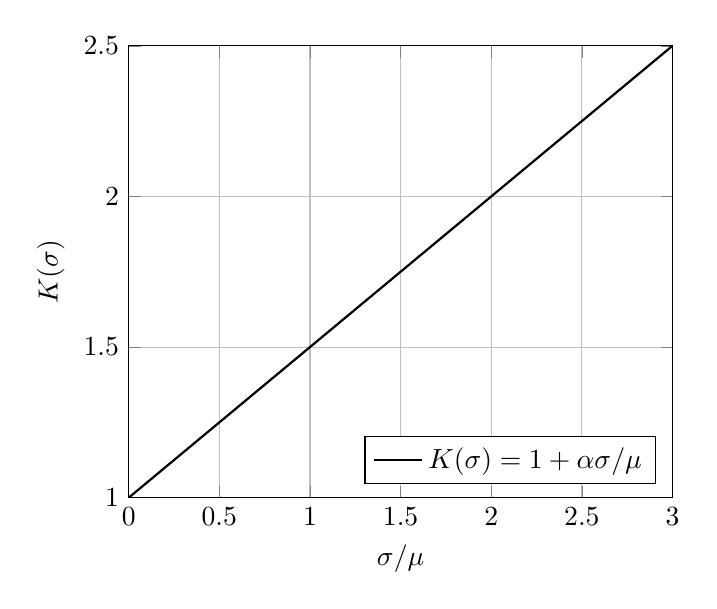
\begin{tikzpicture}
        \begin{axis}[
            width=0.7\textwidth,
            xlabel={$\sigma / \mu$},
            ylabel={$K(\sigma)$},
            xmin=0, xmax=3,
            ymin=1, ymax=2.5,
            domain=0:3,
            samples=200,
            grid=both,
            legend style={at={(0.97,0.03)},anchor=south east}
        ]
            \addplot[thick]
                {1 + 0.5 * x}; % alpha = 0.5
            \addlegendentry{$K(\sigma) = 1 + \alpha \sigma/\mu$}
        \end{axis}
    \end{tikzpicture}
    \caption{Illustrative flux--dependent gauge kinetic function
    $K(\sigma)$ as a function of $\sigma/\mu$, using the linear
    form in Eq.~\eqref{eq:K_sigma_linear} with $\alpha = 0.5$.
    In the full model, $\alpha$ and the functional form of $K$
    can be constrained by jet observations.}
    \label{fig:Ksigma_profile}
\end{figure}

A simple proxy for the jet power in Blandford--Znajek--type
mechanisms is
\begin{equation}
    P_{\mathrm{jet}} \propto K(\sigma)^2 B^2 \Omega_{\mathrm{H}}^2,
\end{equation}
where $B$ is the magnetic field threading the horizon and
$\Omega_{\mathrm{H}}$ is the angular frequency of the black hole
horizon. Holding $B$ and $\Omega_{\mathrm{H}}$ fixed, the dependence
on the flux field enters purely via $K(\sigma)$.\footnote{In a more
complete treatment, $B$ will itself depend on the accretion flow and
possibly on $\sigma$, but the present toy scaling suffices to show
how a single flux degree of freedom can modulate jet power.}

Using the linear form \eqref{eq:K_sigma_linear}, the jet power
scales as
\begin{equation}
    P_{\mathrm{jet}}(\sigma)
    =
    P_0 \left[1 + \alpha \frac{\sigma}{\mu}\right]^2,
    \label{eq:Pjet_sigma}
\end{equation}
with $P_0$ a normalisation that absorbs $B^2 \Omega_{\mathrm{H}}^2$
and geometric factors. Figure~\ref{fig:Pjet_profile} displays this
scaling for a fiducial choice of parameters.

\begin{figure}[t]
    \centering
    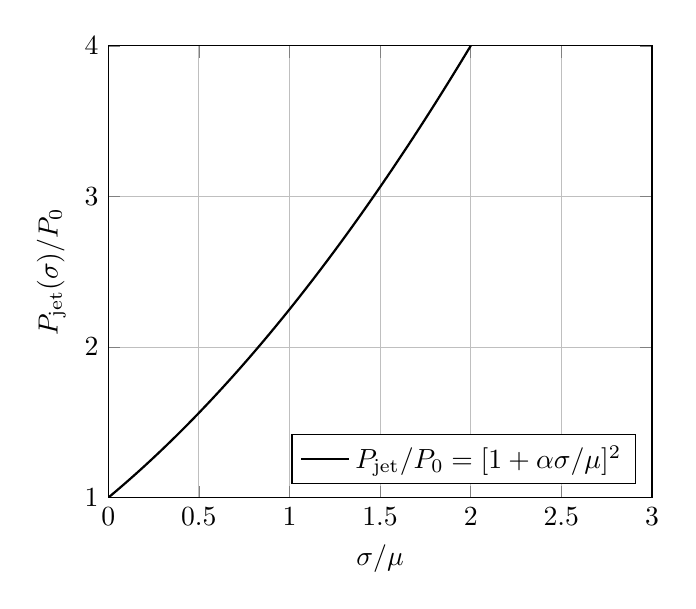
\begin{tikzpicture}
        \begin{axis}[
            width=0.7\textwidth,
            xlabel={$\sigma / \mu$},
            ylabel={$P_{\mathrm{jet}}(\sigma)/P_0$},
            xmin=0, xmax=3,
            ymin=1, ymax=4,
            domain=0:3,
            samples=200,
            grid=both,
            legend style={at={(0.97,0.03)},anchor=south east}
        ]
            \addplot[thick]
                {(1 + 0.5 * x)^2}; % alpha = 0.5
            \addlegendentry{$P_{\mathrm{jet}}/P_0 = [1 + \alpha \sigma/\mu]^2$}
        \end{axis}
    \end{tikzpicture}
    \caption{Illustrative jet power scaling as a function of the
    flux field, using Eq.~\eqref{eq:Pjet_sigma} with $\alpha = 0.5$.
    Even modest variations in the local flux state can, in this toy
    model, generate order-unity changes in jet power at fixed
    accretion rate and black-hole spin.}
    \label{fig:Pjet_profile}
\end{figure}

These plots are not intended as fits to specific objects, but as a
visual proof-of-principle: within the flux--scalar framework the
same degree of freedom $\sigma$ that drives cosmological acceleration
can, via $K(\sigma)$, modulate the efficiency with which black holes
launch relativistic jets.

\section{Local tests: effective gravity and the lunar orbit}
\label{sec:lunar}

Beyond background cosmology, the flux picture can feed into an
effective Newton's constant $G_{\mathrm{eff}}(t)$ relevant for local
dynamics. In the simplest toy implementation used here, the
cosmological flux fraction $\Phi / S_{\max}$ is computed from a
separate entropy-like variable and then mapped to $G_{\mathrm{eff}}$
via
\begin{equation}
    G_{\mathrm{eff}}(t)
    = G_0 \left[1 + g_1 \, f_{\mathrm{flux}}(t)\right],
\end{equation}
where $g_1$ is a dimensionless coupling and $f_{\mathrm{flux}}$ is a
bounded function constructed from the flux deficit or fraction in the
cosmological sector.

As a concrete local test we consider the Earth--Moon system as a
two-body problem with a slowly varying $G_{\mathrm{eff}}(t)$ plus a
phenomenological tidal torque. In a circular-orbit approximation,
the orbital radius $R(t)$ responds to both the tidal gain in angular
momentum and the secular drift in $G_{\mathrm{eff}}$. The toy model
used in this work calibrates the tidal torque to reproduce the
observed $3.8$ cm/yr lunar recession while allowing for an additional,
subdominant contribution from $G_{\mathrm{eff}}(t)$.

\subsection{Lunar orbit model: variable gravity and tidal torque}
\label{subsec:lunar_equations}

The Earth--Moon toy model used in this work is deliberately simple:
we work with a dimensionless system in which
\[
G_0 = 1, \qquad R_0 = 1, \qquad M_{\oplus} = 1, \qquad
M_{\rm M} = 0.0123,
\]
where $R_0$ is the current mean Earth--Moon distance and
$M_{\oplus}, M_{\rm M}$ are the Earth and Moon masses respectively.
Time is measured in years and the integration runs for $T_{\max} =
50$\,yr with time step $\Delta t = {\rm d}t$.

The model couples a slowly varying effective Newton's constant
$G_{\rm eff}(t)$, obtained from the cosmological flux sector, to a
Keplerian two-body problem plus a phenomenological tidal torque that
drives the observed recession.

% ------------------------------------------------
\subsubsection*{Keplerian orbit with $G_{\rm eff}(t)$}

Let $\bm{r}(t) = (x(t),y(t))$ be the Moon's position in the orbital
plane and $R(t) = |\bm{r}(t)|$ the orbital radius. At each time step,
the effective Newton's constant is computed from the flux fraction
$\phi_{\rm flux}(t)$,
\begin{equation}
    G_{\rm eff}(t) = G_0 \left[1 + g_1\,\phi_{\rm flux}(t)\right],
    \label{eq:Geff_lunar}
\end{equation}
where $g_1$ is a small dimensionless coupling fixed elsewhere in the
cosmological model. The gravitational acceleration is then purely
Newtonian with $G_0 \to G_{\rm eff}(t)$:
\begin{align}
    \ddot{\bm{r}}(t)
    &= - \frac{G_{\rm eff}(t)\,M_{\oplus}}{R(t)^3}\,\bm{r}(t),
    \label{eq:newton_vector}\\[3pt]
    \ddot{x}
    &= - \frac{G_{\rm eff}(t)\,M_{\oplus}}{R^3}\,x,
    \qquad
    \ddot{y}
    = - \frac{G_{\rm eff}(t)\,M_{\oplus}}{R^3}\,y.
\end{align}
These equations are integrated with a simple explicit scheme in the
code (velocity and position updates per time step).

% ------------------------------------------------
\subsubsection*{Tidal torque and angular momentum gain}

On top of the variable gravity, we include a phenomenological tidal
torque that transfers angular momentum from the Earth's spin to the
Moon's orbit. The code models this as a secular gain in the Moon's
orbital angular momentum $L$,
\begin{equation}
    \dot{L} = \tau_{\rm tide}(t)
    = \tau_0 \,\frac{M_{\oplus} M_{\rm M}}{R(t)^2}\,G_{\rm eff}(t),
    \label{eq:Ldot_tidal}
\end{equation}
where $\tau_0$ is a dimensionless ``tidal\_torque\_factor'' later
calibrated to reproduce the observed recession rate.

For convenience the numerical implementation works with the specific
angular momentum
\begin{equation}
    h(t) \equiv \frac{L(t)}{M_{\rm M}}
    = R^2 \dot{\phi},
\end{equation}
so that Eq.~\eqref{eq:Ldot_tidal} becomes
\begin{equation}
    \dot{h}(t)
    = \frac{\dot{L}}{M_{\rm M}}
    = \tau_0 \,\frac{M_{\oplus}}{R(t)^2}\,G_{\rm eff}(t).
    \label{eq:hdot_tidal}
\end{equation}
In the code this is implemented via a discrete update
\begin{equation}
    h(t + \Delta t)
    = h(t) + \dot{h}(t)\,\Delta t.
\end{equation}

% ------------------------------------------------
\subsubsection*{Mapping to the semi-major axis and $R(t)$}

Assuming a nearly circular orbit, the semi-major axis $a_{\rm orb}$ is
related to the specific angular momentum by the usual Keplerian
relation with $G_{\rm eff}(t)$,
\begin{equation}
    h^2(t)
    = G_{\rm eff}(t)\,M_{\oplus}\,a_{\rm orb}(t).
    \label{eq:kepler_circular}
\end{equation}
Solving for $a_{\rm orb}$ gives
\begin{equation}
    a_{\rm orb}(t)
    = \frac{h^2(t)}{G_{\rm eff}(t)\,M_{\oplus}}.
    \label{eq:a_from_h}
\end{equation}
In the code we identify $R(t) \simeq a_{\rm orb}(t)$ and use
Eq.~\eqref{eq:a_from_h} to compute a ``new'' radius $R_{\rm new}$ after
each torque update. The instantaneous orbit $(x,y,\dot{x},\dot{y})$ is
then rescaled to this new radius:
\begin{align}
    R_{\rm new}(t) &= \frac{h^2(t)}{G_{\rm eff}(t)\,M_{\oplus}},\\
    s(t)           &= \frac{R_{\rm new}(t)}{R(t)},\\
    \bm{r}         &\to s(t)\,\bm{r},\\
    \dot{\bm{r}}   &\to \sqrt{s(t)}\,\dot{\bm{r}},
\end{align}
which preserves the phase of the orbit while enforcing the updated
Keplerian relation.

% ------------------------------------------------
\subsubsection*{Recession rate and comparison to data}

The primary observable extracted from the simulation is the fractional
recession rate of the Earth--Moon distance,
\begin{equation}
    \Gamma \equiv \frac{1}{R}\frac{\dd R}{\dd t}.
\end{equation}
In practice, the code estimates $\Gamma$ over the full integration
interval $[0,T_{\max}]$ as
\begin{equation}
    \Gamma_{\rm num}
    \simeq
    \frac{R(T_{\max}) - R(0)}{R(0)\,T_{\max}}.
    \label{eq:gamma_num}
\end{equation}
The tidal torque normalisation $\tau_0$ is then calibrated so that
$\Gamma_{\rm num}$ matches the observed value corresponding to a
physical recession of $\simeq 3.8$\,cm/yr at the current distance
$R_0$,
\begin{equation}
    \Gamma_{\rm obs}
    = \frac{(3.8~{\rm cm/yr})}{R_0}
    \simeq 10^{-10}~{\rm yr}^{-1}.
\end{equation}
Because the model is linear in $\tau_0$, we can perform a single
``baseline'' run with a fiducial $\tau_0^{\rm base}$ to measure
$\Gamma_{\rm num}^{\rm base}$, and then set
\begin{equation}
    \tau_0
    = \tau_0^{\rm base}\,
      \frac{\Gamma_{\rm obs}}{\Gamma_{\rm num}^{\rm base}},
\end{equation}
after which the calibrated model reproduces the observed lunar
recession by construction. Any additional contribution from the
time-variation of $G_{\rm eff}(t)$ in Eq.~\eqref{eq:Geff_lunar} is
therefore constrained to be subdominant to the tidal torque within
this toy framework.


% ================================================================
\section{Discussion and outlook}
\label{sec:discussion}

The main gain from working at the level of a covariant
Lagrangian, rather than treating the flux sector as a purely
numerical modification of $H(a)$, is conceptual clarity and
comparability. Once the model is written as
\begin{equation}
    S = \int \dd^4x \sqrt{-g}
    \left[
        \frac{\mpl^2}{2} R
        - \frac{1}{2}(\nabla\sigma)^2
        - V(\sigma)
        + \Lag_{\mathrm{m}} + \Lag_{\mathrm{r}}
    \right],
\end{equation}
it can be placed side by side with standard quintessence, $k$-essence
and many modified-gravity models. This makes it immediately clear
which parts of the dynamics are genuinely new (the flux interpretation
and potential choice) and which parts are recycled from the existing
scalar-field toolkit. It also fixes the stress--energy tensor and the
covariant conservation laws unambiguously, which is essential once one
goes beyond background cosmology.

From the observational point of view, the Lagrangian formulation
provides a natural list of falsifiable predictions. At background
level, the model predicts a specific redshift dependence of the
effective dark-energy equation of state,
\begin{equation}
    w_\sigma(a)
    = \frac{\frac{1}{2}\dot{\sigma}^2 - V(\sigma)}
           {\frac{1}{2}\dot{\sigma}^2 + V(\sigma)},
\end{equation}
and therefore a specific family of expansion histories $H(a)$ once
$(V_0,\mu,\Omega_{m0})$ are fixed by the calibration procedure in
Sec.~\ref{subsec:param_choice}. Any sufficiently precise reconstruction
of $H(a)$ from low-redshift data (BAO, SNe, cosmic chronometers) or
of $w(a)$ from combined CMB+BAO+SNe analyses can in principle rule out
this particular potential shape. Likewise, the requirement that the
model reproduce the CMB acoustic scale $\theta_\star$ and the BAO
distance ladder leaves only a restricted region in the
$(V_0,\mu,\Omega_{m0})$ space; future tightening of these geometric
constraints will either further shrink this region or exclude the
model.

Beyond the homogeneous background, the next layer of falsifiable
predictions comes from perturbations and structure growth. Once the
flux field is treated as a genuine dynamical scalar, its linear
perturbations obey a Klein--Gordon equation on the perturbed FLRW
background, and feed into the Poisson equation via their
contribution to the total stress--energy tensor. This leads to a
modified growth history $f(a) = \dd\ln D / \dd\ln a$ and a
predicted growth index $\gamma$ that can be tested against redshift
space distortion measurements and weak lensing surveys. In that
sense, the flux--scalar model is not just a re-labelling of
$\Lambda$CDM but a definite point in the broader space of dark
energy / modified gravity theories that will be probed by DESI,
Euclid and LSST.

The flux picture itself suggests several natural extensions that
are left for future work. On the cosmological side, one can move
from background-only to a full perturbation treatment, computing CMB
anisotropies and matter power spectra with the flux scalar included
as an explicit degree of freedom rather than an effective $w(a)$.
On the high-energy side, the black--hole + jet toy model sketched in
Sec.~\ref{sec:bh_jet} could be developed into a separate, more
detailed paper, exploring whether a single flux field $\sigma$ can
consistently modulate both cosmological acceleration and jet
efficiencies in realistic Kerr geometries. Finally, a key conceptual
step will be to connect the entropy / flux deficit variables used in
the numerical experiments directly to $\sigma$, rather than treating
them as parallel bookkeeping devices. That would turn the current
collection of ``toys'' into a single, coherent flux framework in
which cosmology, black-hole phenomenology and local tests such as
the Earth--Moon system all emerge from one underlying dynamical
field.


\paragraph{Key points.}
This first paper has three main goals:
\begin{enumerate}
    \item Define the flux--scalar model at the level of a covariant
    action with an explicit potential.
    \item Show that it reduces to a numerically tractable set of
    background equations, recovering standard behaviour in appropriate
    limits.
    \item Illustrate how the same framework can be confronted with
    both high-redshift (CMB) and low-redshift (local orbital) data.
\end{enumerate}

Future work will lift several of the simplifying assumptions made
here, including the treatment of perturbations, a more realistic
mapping between flux variables and $G_{\mathrm{eff}}$, and detailed
comparisons with large-scale structure data.

% ================================================================
\section*{Acknowledgements}

The author thanks various online tools and numerical experiments
for assistance in exploring and testing the flux--scalar model.

% ================================================================
\bibliographystyle{unsrt}
\begin{thebibliography}{99}

\bibitem{quintessence_review}
P.~J.~E.~Peebles and B.~Ratra,
\newblock ``The cosmological constant and dark energy,''
\newblock {\em Rev. Mod. Phys.} \textbf{75}, 559 (2003).

\bibitem{copeland_review}
E.~J.~Copeland, M.~Sami and S.~Tsujikawa,
\newblock ``Dynamics of dark energy,''
\newblock {\em Int. J. Mod. Phys. D} \textbf{15}, 1753 (2006).

% TODO: Add your own references and any data / code DOIs once you publish them.

\end{thebibliography}

\end{document}
